\documentclass[a4paper, 11pt]{article}
\usepackage{hyperref}
\usepackage[margin=0.5in]{geometry}

\usepackage{amsmath}
\usepackage[arrowdel]{physics}
\usepackage{graphicx}
\usepackage{subfig}

\newcommand{\kb}{\ensuremath{k_{\text{B}}}}
\newcommand{\Na}{\ensuremath{N_{\text{A}}}}
\newcommand{\cc}[1]{#1^{\star}}
\newcommand{\adj}[1]{#1^{\dagger}}
\newcommand{\commut}[2]{[#1, #2]}
\newcommand{\cdir}[1]{\ensuremath{\left[#1\right]}}
\newcommand{\cplane}[1]{\ensuremath{\left(#1\right)}}
\newcommand{\cpset}[1]{\ensuremath{\left\{#1\right\}}}
\newcommand{\del}[3][]{\partial_{#2}^{#1}#3}
\newcommand{\deval}[4][]{\eval{\dv[#1]{#2}{#3}}_{#4}}
\newcommand{\pdeval}[4][]{\eval{\del[#1]{#2}{#3}}_{#4}}
\newcommand{\integ}[5][]{\int\limits_{#2}^{#3}\dd[#1]{#4}#5}

\title{Summary of SK2758 Solid State Physics}
\author{Yashar Honarmandi \\ yasharh@kth.se}
\date{\today}

\begin{document}

\maketitle

\begin{abstract}
	Detta ær en sammanfattning av kursen SH1014 Modern fysik.
\end{abstract}

\pagenumbering{roman}
\thispagestyle{empty}

\newpage

\tableofcontents

\newpage

\pagenumbering{arabic}

\section{Crystals}

\paragraph{Crystals}
Solid state physics, as we will study it, is concerned with crystals. A crystal is an arrangement of atoms which is repeated periodically. When developing the physics of crystals, we will assume their repetition to be infinite.

\paragraph{Basis}
The arrangement of atoms which is repeated in a crystal is termed the basis.

\paragraph{Lattices}
The set of points to which the basis is attached is termed the lattice.

\paragraph{Bravais Lattices}
A Bravais lattice is a lattice such that the arrangement of lattice points looks exactly equal from any lattice point. This turns out to be equivalent to the lattice being infinite and symmetric under certain discrete translations. We will treat crystal lattices as Bravais lattices.

The two-dimensional Bravais lattices are the rectangular,

\begin{figure}[!ht]
	\centering
	\subfloat[Square.]
	{
		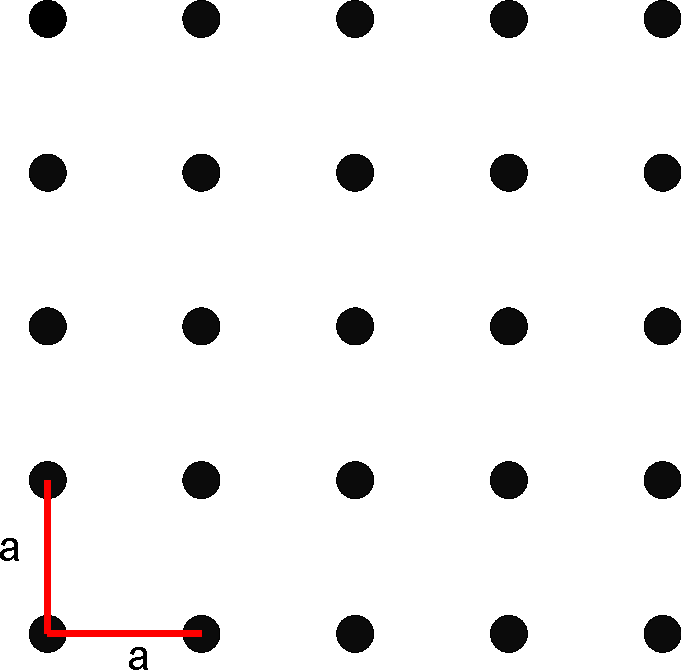
\includegraphics[width = 0.3\textwidth]{./Images/2d_square.pdf}
	}
	\hfil
	\subfloat[Rectangular.]
	{
		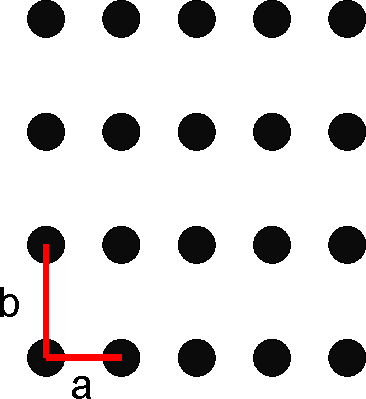
\includegraphics[width = 0.3\textwidth]{./Images/2d_rectangular.pdf}
	}
\end{figure}

%TODO: Add 2D and 3D Bravais lattices

\paragraph{Lattice Vectors}
The set $\{\vb{a}_{i}\}$ of lattice vectors of a Bravais lattice is the smallest possible set of vectors such that translating the lattice by $u_{i}\vb{a}_{i}$, where the $u_{i}$ are integers, leaves the lattice unchanged. There is an infinite number of ways to define the lattice vectors of a given lattice.

\paragraph{Primitive Lattice Vectors}
A set of lattice vectors is primitive if any two equivalent points are connected by integer combinations of the lattice vectors.

\paragraph{Crystal Axes}
The crystal axes are a set of directions that span space. These may be chosen according to, for instance, the primitive lattice vectors or other directions connected to the symmetry of the lattice.

\paragraph{Crystal Cell}
The crystal cell is the repeat unit of the crystal. It may be constructed in an infinite number of ways.

\paragraph{Lattice Constants}
Lattice constants are a set of parameters defining the dimensions of the cell.

\paragraph{Primitive Cell}
The primitive cell is a minimum-volume cell. It contains only one lattice point, and is thus termed a unit cell. Its infinite translation throughout space yields the lattice.

\paragraph{Primitive Basis}
The primitive basis is the basis associated with the primitive cell.

\paragraph{Wigner-Seitz Cell}
The Wigner-Seitz Cell is the cell constructed by for any lattice point dividing space into two at the middle of and normal to the line between the point in question and all other points, and choosing the smallest possible region of space containing the point from this.

\paragraph{Lattice Point Group}
The lattice point group is the group of operations which, applied about a lattice point (i.e. keeping this point fixed), leaves the lattice unchanged. Examples of possible fundamental operations include:
\begin{itemize}
	\item rotations.
	\item reflections.
\end{itemize}

\paragraph{Lattice Space Group}
The space group of the Bravais lattices is the group of symmetries of all Bravais lattices of a given dimensionality. It contains both point groups and translations.

\paragraph{$n$-Fold Rotations}
An $n$-fold rotation is a rotation operation such that it reduces to the identity operation when applied $n$ times. Lattices cannot be symmetric under $5$-fold rotation.

\paragraph{Crystal Planes}
In a cell it is useful to define crystallographic planes. These are indicated by a set of indices \cplane{hkl}, the computation of which we will return to. A bar above any element indicates that element to be negative.

A set of parallel planes such that all lattice points are contained in the set may be denoted \cpset{hkl}.

\paragraph{Crystallographic Directions}
Likewise we define crystallographic directions by the notation \cdir{uvw}. The indices are the set of the smallest integers such that they form a vector parallel to the one in question.

\paragraph{Random Stacking}
Randomly stacked crystals are formed by densely packed layers of atoms being stacked without long-range order in the stacking direction.

\paragraph{Polytopism}
Polytopism is a milder variation of random stacking, where the order of the stacked layers is extremely long-range.

%TODO: Add special structures

\paragraph{X-Ray Diffraction}
X-ray diffraction is the process of shining X-rays onto a material in order to characterize it. Before atomic physics, it was discovered that solids scattered X-rays intensely in specific directions, as opposed to light, which was reflected by the solid. In the context of solid-state physics, we can interpret this as crystal planes acting as diffraction grids that scatter the X-rays. This interpretation makes sense because the wavelength of X-rays is comparable to interatomic distances in a solid, consistent with the regime in which classical wave physics predicts that diffraction phenomena are significant, and the scattered light being localized is consistent with diffraction of other waves.

\paragraph{Bragg's Law}
Bragg's law was a first attempt at explaining X-ray diffraction patterns. To derive it, consider a solid composed of aligned and stacked atomic planes separated by a distance $d$ on which electromagnetic radiation of wavelength $\lambda$ is incident at angle $\theta$ to the planes, and suppose each plane reflects the radiation specularly (following the law of reflection) and elastically (preserving the wavelength). Comparing radiation reflected from two adjacent layers, the light in the lower layer travels a distance $2d\sin{\theta}$ longer. In order for the radiation from these layers to interfere constructively, we must have
\begin{align*}
	2d\sin{\theta} = n\lambda,\ n = 1, 2, \dots
\end{align*}
This is Bragg's law. It is a very rough description of X-ray diffraction, but predicts the phenomenology correctly. It also predicts that diffraction occurs for $\lambda < 2d$, which is why light, for instance, is not diffracted by solids.

\paragraph{Fourier Analysis and Reciprocal Space}
The translational symmetry of the lattice implies that the tools of Fourier analysis are applicable when studying solid-state physics. Any observable $A$ defined on the crystal lattice may be written as
\begin{align*}
	A = \sum\limits_{\vb{G}}A_{\vb{G}}e^{i\vb{G}\cdot\vb{r}}.
\end{align*}
The coefficients in the series expansion are given by
\begin{align*}
	A_{\vb{G}} = \frac{1}{V_{\text{cell}}}\integ[d]{\text{cell}}{}{\vb{r}}{A(\vb{r})e^{-i\vb{G}\cdot\vb{r}}}.
\end{align*}
In order for $A$ to be an observable, we must have $A_{-\vb{G}} = \cc{A_{\vb{G}}}$. The fact that $A$ is an observable on the crystal lattice implies that it must have the same symmetries - in particular translational symmetry. This implies
\begin{align*}
	A(\vb{r} + u_{i}\vb{a}_{i}) = A(\vb{r}) \implies u_{i}\vb{G}\cdot\vb{a}_{i} = 2\pi n
\end{align*}
where $n$ is an integer. The vectors $\vb{G}$ must have reciprocal length as their dimension, and are thus vectors in what is termed reciprocal space.

\paragraph{The Reciprocal Lattice}
The simplest choice of vectors satisfying
\begin{align*}
	u_{i}\vb{G}\cdot\vb{a}_{i} = 2\pi n
\end{align*}
is integer combinations of a set of vectors $\{\vb{b}_{i}\}$ such that $\vb{a}_{i}\cdot\vb{b}_{j} = 2\pi\delta_{ij}$. The set of vectors $\{\vb{b}_{i}\}$ thus defines a Bravais lattice in reciprocal space, termed the reciprocal lattice. In three dimensions, the explicit formula for the reciprocal lattice vectors is
\begin{align*}
	\vb{b}_{1} = \frac{2\pi}{V_{\text{cell}}}\vb{a}_{2}\times\vb{a}_{3},\ V_{\text{cell}} = \vb{a}_{1}\cdot(\vb{a}_{2}\times\vb{a}_{3})
\end{align*}
with cyclic permutation of the indices yielding the other two.

\paragraph{Crystal Planes and the Reciprocal Lattice}
Assume that there is a lattice point in the origin and that the closest crystal plane with orientation specified by the normal vector $\vb{n}$ is a distance $d$ from the origin. Any plane parallel to the plane in question is described by
\begin{align*}
	\vb{r}\cdot\vb{n} = md,\ m = 0, \pm 1, \dots
\end{align*}

Consider now a translation by $\vb{T}$ such that the lattice is left invariant. Assuming the translation to be between lattice points, the translation must satisfy the equation of some crystal plane, implying
\begin{align*}
	\vb{T}\cdot\vb{n} = md.
\end{align*}
In particular, if the translation is to a point in a plane adjacent to the origin, we have
\begin{align*}
	\vb{T}\cdot\frac{2\pi}{d}\vb{n} = 2\pi.
\end{align*}
Comparing this to the definition of the reciprocal lattice implies that the plane is normal to a reciprocal lattice vector
\begin{align*}
	\vb{G} = \frac{2\pi}{d}\vb{n}.
\end{align*}
This is the shortest reciprocal lattice vector describing the plane. The expression above implies
\begin{align*}
	d = \frac{2\pi}{\abs{\vb{G}}}.
\end{align*}

\paragraph{Miller Indices}
Returning to the indexing system for crystal planes, we may decompose the normal vector as
\begin{align*}
	\vb{G} = h\vb{b}_{1} + k\vb{b}_{2} + l\vb{b}_{3}.
\end{align*}
These indices are exactly the indices used to describe a crystal plane, and are termed Miller indices. As $\vb{G}$ is the shortest vector describing the plane, the indices cannot contain any common factors.

The Miller indices may also be computed from the real lattice according to the following rules:
\begin{enumerate}
	\item For each axis, defined by the lattice vectors, identify the intercepts of the plane with the axis as units of the lattice parameters.
	\item Compute the reciprocals of each intercept.
	\item Reduce to three integers with the same ratio.
\end{enumerate}

\paragraph{Interplanar Distances}
Consider the set of \cpset{hkl} planes. We are interested in computing the distance between two adjacent such planes. To do this, we will first need a unit normal to any such plane. According to the construction of the Miller indices, the vectors
\begin{align*}
\vb{v}_{1} = \frac{1}{h}\vb{a}_{1} - \frac{1}{k}\vb{a}_{2},\ \vb{v}_{2} = \frac{1}{h}\vb{a}_{1} - \frac{1}{l}\vb{a}_{3}
\end{align*}
span the plane, apart from some constant spatial shift. Hence we are interested in a vector that is simultaneously normal to both of these. One possible choice is
\begin{align*}
	\vb{G}_{hkl} = h\vb{b}_{1} + k\vb{b}_{2} + l\vb{b}_{3}.
\end{align*}
From this, obtaining a unit normal is trivial. Next we need a vector from one plane to the other. One possible choice is
\begin{align*}
	\vb{T} = \frac{1}{h}\vb{a}_{1},
\end{align*}
as one cell has space for $h$ planes of this type when counted along the $\vb{a}_{1}$ direction. From this, the distance is given by
\begin{align*}
	d = \frac{1}{\abs{\vb{G}_{hkl}}}\vb{G}_{hkl}\cdot\vb{T} = \frac{2\pi}{\abs{\vb{G}_{hkl}}},
\end{align*}
which is true for any Bravais lattice.

\paragraph{Diffraction by Solids}
Using the language of Fourier analysis and reciprocal space, we will try to derive a more sophisticated diffraction condition.

To do this, consider a crystal exposed to far-field radiation described by a wave vector $\vb{k}$ which is scattered elastically by the crystal in an arbitrary direction and observed in the far-field region in some direction, in which the wave vector is $\vb{k}^{\prime}$. Considering the interference between two points displaced by $\vb{r}$, the phase difference between the radiation from the two points is $(\vb{k} - \vb{k}^{\prime})\cdot\vb{r}$. Supposing that the amplitude of the scattered wave is proportional to the electron density (or, really, any property defined on the lattice), the total scattered amplitude is proportional to the (confusingly termed) scattering amplitude
\begin{align*}
	F = \integ[d]{}{}{\vb{r}}{n(\vb{r})e^{i(\vb{k} - \vb{k}^{\prime})\cdot\vb{r}}}.
\end{align*}
Adding the series expansion of the electron density yields
\begin{align*}
	F = \integ[d]{}{}{\vb{r}}{\sum\limits_{\vb{G}}n_{\vb{G}}e^{i\vb{G}\cdot\vb{r}}e^{-i\Delta\vb{k}\cdot\vb{r}}} = \integ[d]{}{}{\vb{r}}{\sum\limits_{\vb{G}}n_{\vb{G}}e^{i(\vb{G} - \Delta\vb{k})\cdot\vb{r}}} = \sum\limits_{\vb{G}}\integ[d]{}{}{\vb{r}}{n_{\vb{G}}e^{i(\vb{G} - \Delta\vb{k})\cdot\vb{r}}}.
\end{align*}
For the case $\Delta\vb{k} = \vb{G}$ for any one particular reciprocal lattice vector, the exponential in this term vanishes, leaving a term $Vn_{\vb{G}}$. It can be shown that all other terms in the scattering amplitude vanish, yielding $F = Vn_{\vb{G}}$ for this case and $F = 0$ otherwise. The most fundamental diffraction condition is thus
\begin{align*}
	\Delta\vb{k} = \vb{G}.
\end{align*}

While we have in principle obtained a diffraction condition now, we can simplify it by using the fact that the scattering is inelastic. We obtain
\begin{align*}
	2\vb{k}\cdot\vb{G} + G^{2} = 0.
\end{align*}
It may be rewritten by swapping $\vb{G}$ for $-\vb{G}$, which is also a reciprocal lattice vector, to yield
\begin{align*}
	2\vb{k}\cdot\vb{G} = G^{2}.
\end{align*}

Note that this implies that information about the reciprocal lattice, and therefore the lattice itself, may be obtained from diffraction experiments.

\paragraph{Laue's Equations}
The fundamental diffraction criterion implies
\begin{align*}
	\Delta\vb{k}\cdot\vb{a}_{i} = 2\pi v_{i}
\end{align*}
for some integer $v_{i}$, simultaneously for all lattive vectors. This implies that reflections are only found at the intersection of three cones in reciprocal space. This is very strict, and such reflections must be found by sweeping in crystal orientation and/or wavelength or by chance.

\paragraph{The Ewald Sphere}
The Ewald sphere is a tool for visualizing the necessary conditions for diffractions. To construct it, draw the incident wave vector starting in a point such that it terminates in a reciprocal lattice point. From the starting point, draw a sphere of radius $k$. All reciprocal lattice points corresponding to a diffraction peak are found on this sphere.

\paragraph{Brillouin Zones}
To introduce the concept of Brillouin zones, rewrite the diffraction condition as
\begin{align*}
	\vb{k}\cdot\frac{1}{2}\vb{G} = \left(\frac{1}{2}G\right)^{2}.
\end{align*}
For a fixed $\vb{G}$, this equation defines the set of wave vectors terminating on the bisector of $\vb{G}$. This is similar to the construction of the Wigner-Seitz cell in real space, but now extended to construct zones using all points in the reciprocal lattice. Constructing these bisectors divides the reciprocal space into Brillouin zones (a single Brillouin zone is the combinations of all zones a fixed number of zones from the central zone). The central zone, which is the Wigner-Seitz cell in reciprocal space, is the first Brillouin zone.

\paragraph{Volume of the Brillouin Zone}
We would like to compute the volume of the Brillouin zone in terms of the volume of the unit cell. To do this, we note that the unit cell volume is given by
\begin{align*}
	V_{\text{c}} = \vb{a}_{1}\cdot(\vb{a}_{2}\times\vb{a}_{3}).
\end{align*}
Using this, the volume of the Brillouin zone is given by
\begin{align*}
	V_{\text{r}} = \vb{b}_{1}\cdot(\vb{b}_{2}\times\vb{b}_{3}).
\end{align*}
The vector in the parenthesis is given by
\begin{align*}
	\vb{b}_{2}\times\vb{b}_{3} &= \frac{(2\pi)^{2}}{V_{\text{c}}^{2}}(\vb{a}_{3}\times\vb{a}_{1})\times (\vb{a}_{1}\times\vb{a}_{2}) \\
	                           &= \frac{(2\pi)^{2}}{V_{\text{c}}^{2}}((\vb{a}_{3}\cdot(\vb{a}_{1}\times\vb{a}_{2}))\vb{a}_{1} - (\vb{a}_{3}\cdot(\vb{a}_{1}\times\vb{a}_{1}))\vb{a}_{2}) \\
	                           &= \frac{(2\pi)^{2}}{V_{\text{c}}}\vb{a}_{1},
\end{align*}
and thus the volume of the Brillouin zone is given by
\begin{align*}
	V_{\text{r}} = \frac{(2\pi)^{3}}{V_{\text{c}}}.
\end{align*}

\paragraph{The Structure Factor and Atomic Form Factor}
When the diffraction condition is satisfied, i.e. $\Delta\vb{k} = \vb{G}$ for some reciprocal lattice vector, the scattering amplitude for a crystal of $N$ cells becomes
\begin{align*}
	F = \integ[d]{}{}{\vb{r}}{n(\vb{r})e^{-i\vb{G}\cdot\vb{r}}} = N\integ[d]{\text{cell}}{}{\vb{r}}{n(\vb{r})e^{-i\vb{G}\cdot\vb{r}}} = NS_{\vb{G}},
\end{align*}
where we have introduced the structure factor $S_{\vb{G}}$, which describes the effect of the electron distribution in the cell on the scattering amplitude for a given diffraction peak.

Writing the electron density as a superposition of contributions from each atom in the basis (this decomposition is not unique, but somehow this is not a problem), we obtain
\begin{align*}
	S_{\vb{G}} = \integ[d]{\text{cell}}{}{\vb{r}}{\sum n_{j}(\vb{r} - \vb{r}_{j})e^{-i\vb{G}\cdot\vb{r}}}
\end{align*}
where the $\vb{r}_{j}$ are the positions of the atoms in the basis. We rewrite this as
\begin{align*}
	S_{\vb{G}} = \sum\integ[d]{\text{cell}}{}{\vb{r}}{n_{j}(\vb{r} - \vb{r}_{j})e^{-i\vb{G}\cdot\vb{r}}} = \sum e^{-i\vb{G}\cdot\vb{r}_{j}}\integ[d]{\text{cell}}{}{\vb{r}}{n_{j}(\vb{r})e^{-i\vb{G}\cdot\vb{r}}}
\end{align*}
where the last step follows from the translational symmetry. Defining the atomic form factor
\begin{align*}
	f_{j, \vb{G}} = \integ[d]{\text{cell}}{}{\vb{r}}{n_{j}(\vb{r})e^{-i\vb{G}\cdot\vb{r}}}
\end{align*}
we have
\begin{align*}
	S_{\vb{G}} = \sum f_{j, \vb{G}}e^{-i\vb{G}\cdot\vb{r}_{j}}.
\end{align*}

When observing electron distributions in solids, these appear close to those of free atoms. This does not mean that electrons are not distributed in a solid versus for free atoms, but that these corrections do not have a major effect on the atomic form factors. Thus it may be relevant to write these as
\begin{align*}
	f_{j, \vb{G}} = \integ[d]{}{}{\vb{r}}{n_{j}(\vb{r})e^{-i\vb{G}\cdot\vb{r}}}
\end{align*}
where the electron distribution is that of a free atom and the integration is performed over all of space.

The construction of the structure factor is not unique, and may be performed for any repeat unit in the crystal. This is handy as it can simplify many computations. For example, considering a face-centered cubic structure, it can be considered as a simple cubic structure with three atoms in the basis or as an FCC structure such that summation must be performed over the entire conventional cell.

\section{Phonons and Crystal Vibration}

\paragraph{The Monoatomic Chain}
Vibrations in a crystal lattice along a certain crystal direction are vibrations along a chain of atoms lying in that direction. Hence we will need to understand the (classical) physics of particles on chains.

%TODO: Show without assuming x dependence
Consider a chain of atoms at positions $x_{n} = na + u_{n}$, the first term of which is the equliibrium position and the second is the fluctuations from equilibrium. Assuming a harmonic potential with intensity $C$ between nearest neighbours in the chain, your favorite choice of equations of motion will yield
\begin{align*}
	m\dv[2]{x_{n}}{t} = m\dv[2]{u_{n}}{t} = C(x_{n + 1} - x_{n}) - C(x_{n} - x_{n - 1}) = C(x_{n + 1} + x_{n - 1} - 2x_{n}) = C(u_{n + 1} + u_{n - 1} - 2u_{n}).
\end{align*}
When studying lattice vibrations, we are interested in solutions to the equations of motion which are travelling waves, of the form
\begin{align*}
	u_{n} = u_{0}e^{i(Kna - \omega t)}.
\end{align*}
Inserting this into the equations of motion yields
\begin{align*}
	-m\omega^{2}u_{0}e^{i(Kna - \omega t)} = Cu_{0}e^{i(Kna - \omega t)}\left(e^{iKa} + e^{-iKa} - 2\right) = 2Cu_{0}e^{i(Kna - \omega t)}\left(\cos{Ka} - 1\right) = -4Cu_{0}e^{i(Kna - \omega t)}\sin[2](\frac{Ka}{2}).
\end{align*}
This implies the dispersion relation
\begin{align*}
	\omega = \sqrt{\frac{4C}{m}}\abs{\sin(\frac{Ka}{2})}.
\end{align*}

To continue our study, we introduce
\begin{align*}
	\xi = \frac{Ka}{2\pi},\ \omega_{0} = \sqrt{\frac{4C}{m}},
\end{align*}
allowing us to write the dispersion relation as
\begin{align*}
	\omega = \omega_{0}\abs{\sin(\pi\xi)}.
\end{align*}
Firstly we note that the dispersion relation has a period of $\pi$ in the new coordinates. In addition, we note that $\xi$ for this chain is a measure of progression in the reciprocal lattice - each integer value of $\xi$ corresponds to a reciprocal lattice point. This means that all of the physics of the chain are contained within the interval $-\frac{1}{2} < \xi < \frac{1}{2}$, which is the first Brillouin zone of the lattice.

The periodicity of the dispersion relation has an interpretation. Suppose that $K = k + \frac{2\pi}{a}$ where $k$ is within the first Brillouin zone. The motion of any particle in the chain when exposed to such a wave is given by
\begin{align*}
	u_{n} = u_{0}e^{i(Kna - \omega t)} = u_{0}e^{2\pi ni}e^{i\left(kna - \omega t\right)} = u_{0}e^{i\left(kna - \omega t\right)}.
\end{align*}
Hence the periodicity of the dispersion relation is due to the fact that the travelling wave is only defined at discrete points.

The group velocity of such lattice vibrations is given by
\begin{align*}
	v_{\text{g}} = \dv{\omega}{K} = \frac{1}{2\omega}\dv{\omega^{2}}{K} = \frac{1}{2\omega_{0}\abs{\sin(\pi\xi)}}\cdot \frac{2a\omega_{0}^{2}}{2}\sin(\frac{Ka}{2})\cos(\frac{Ka}{2}) = \frac{1}{2}a\omega_{0}\cos(\pi\xi)\text{sgn}\left(\sin(\pi\xi)\right),
\end{align*}
where the last factor merely describes the direction of propagation. In the long-wavelength limit, close to the origin in reciprocal space, we obtain
\begin{align*}
	\omega \approx \omega_{0}\pi\xi = \frac{1}{2}Ka\omega_{0},\ v_{\text{g}} \approx \frac{1}{2}a\omega_{0},
\end{align*}
implying the linear dispersion relation $\omega = v_{\text{g}}K$. Identifying $Ca$ as a measure of the tension and $\frac{m}{a}$ as the density, we also have
\begin{align*}
	v_{\text{g}} = \sqrt{\frac{T}{\rho}},
\end{align*}
as expected for acoustic waves in a solid. When approaching the Brillouin zone boundary, we obtain
\begin{align*}
	v_{\text{g}} = 0,
\end{align*}
representing a standing wave solution. The wavelength corresponding to the zone boundary is the shortest wavelength that can propagate in the material.

\paragraph{The Diatomic Chain}
To study the effect of the basis, consider a chain of atoms with two atoms in the basis and lattice parameter $a$. Denoting the fluctuations of each type of atom by $u$ and $v$ respectively and only considering nearest-neighbour interactions, the equations of motion are
\begin{align*}
	m_{1}\dv[2]{u_{n}}{t} = C(v_{n} + v_{n - 1} - 2u_{n}),\ m_{2}\dv[2]{v_{n}}{t} = C(u_{n + 1} + u_{n} - 2v_{n}).
\end{align*}
We again look for plane wave solutions of the form
\begin{align*}
	u_{n} = u_{0}e^{i(Kna - \omega t)},\ v_{n} = v_{0}e^{i(Kna - \omega t)}.
\end{align*}
Inserting this into the equations of motion yields
\begin{align*}
	-m_{1}\omega^{2}u_{0}e^{i(Kna - \omega t)} &= C\left(v_{0}e^{i(Kna - \omega t)} + v_{0}e^{i(K(n - 1)a - \omega t)} - 2u_{0}e^{i(Kna - \omega t)}\right) \\
	                                           &= Ce^{-i(Kna - \omega t)}\left(v_{0}\left(1 + e^{-iKa}\right) - 2u_{0}\right), \\
	-m_{2}\omega^{2}v_{0}e^{i(Kna - \omega t)} &= C\left(u_{0}e^{i(K(n + 1)a - \omega t)} + u_{0}e^{i(Kna - \omega t)} - 2v_{0}e^{i(Kna - \omega t)}\right) \\
	                                           &= Ce^{i(Kna - \omega t)}\left(u_{0}\left(e^{iKa} + 1\right) - 2v_{0}\right).
\end{align*}
This is a homogenous system of equations in the amplitudes. A non-trivial solution (corresponding to there being motion in the system) corresponds to the determinant of the coefficient matrix being zero. This implies
\begin{align*}
	\mqty
	[
		2C - m_{1}\omega^{2}       & -C\left(1 + e^{-iKa}\right) \\
		-C\left(e^{iKa} + 1\right) & 2C - m_{2}\omega^{2}
	]
	&= 0, \\
	(2C - m_{1}\omega^{2})(2C - m_{2}\omega^{2}) - C^{2}\left(1 + e^{-iKa}\right)\left(e^{iKa} + 1\right) &= 0, \\
	m_{1}m_{2}\omega^{4} - 2C(m_{1} + m_{2})\omega^{2} + 2C^{2}\left(1 - \cos(Ka)\right) &= 0,
\end{align*}
with solution
\begin{align*}
	\omega^{2} &= \frac{2C(m_{1} + m_{2}) \pm \sqrt{4C^{2}(m_{1} + m_{2})^{2} - 8m_{1}m_{2}C^{2}\left(1 - \cos(Ka)\right)}}{2m_{1}m_{2}}.
\end{align*}
Defining
\begin{align*}
	\omega_{0} = \sqrt{\frac{C(m_{1} + m_{2})}{m_{1}m_{2}}}
\end{align*}
we obtain
\begin{align*}
	\omega^{2} &= \omega_{0}^{2}\left(1 \pm \sqrt{1 - 4\frac{m_{1}m_{2}}{(m_{1} + m_{2})^{2}}\sin[2](\frac{1}{2}Ka)}\right).
\end{align*}
The two choices of sign here represent two so-called branches of the dispersion relation, one termed the optical branch and the other the acoustic branch. The terminology will be clarified later.

We proceed by studying the limiting cases. In the low-wavelength limit we have
\begin{align*}
	\omega^{2} &\approx \omega_{0}^{2}\left(1 \pm \sqrt{1 - \frac{m_{1}m_{2}}{(m_{1} + m_{2})^{2}}(Ka)^{2}}\right) \\
	           &\approx \omega_{0}^{2}\left(1 \pm 1 \mp \frac{m_{1}m_{2}}{2(m_{1} + m_{2})^{2}}(Ka)^{2}\right),
\end{align*}
yielding
\begin{align*}
	\omega_{\text{op}} \approx \sqrt{2}\omega_{0},\ \omega_{\text{ac}} \approx \frac{\sqrt{C}}{\sqrt{2(m_{1} + m_{2})}}\abs{Ka}.
\end{align*}
For the optical branch, we thus obtain
\begin{align*}
	\frac{u_{0}}{v_{0}} = \frac{2C}{2C - 2m_{1}\omega_{0}^{2}} = \frac{2m_{2}}{2m_{2} - 2(m_{1} + m_{2})} = -\frac{m_{2}}{m_{1}},
\end{align*}
and for the acoustic branch we obtain
\begin{align*}
	\frac{u_{0}}{v_{0}} = \frac{2C}{2C - 2m_{1}\frac{C}{2(m_{1} + m_{2})}(Ka)^{2}} \approx 1,
\end{align*}
This reveals the nature of the nomenclature, as acoustic modes correspond to atoms oscillating in phase and propagating acoustic waves, whereas optical modes correspond to atoms being in anti-phase and can thus be excited by electromagnetic waves in ionic crystals.

Simultaneously plotting the dispersion relations of the two branches in the first Brillouin zone yields two different curves. As the anti-phase solution in the low-wavelength limit for the optical branch corresponds to a periodicity of $\lambda = a$ for the motion, we can interpret excitations of oscillations in the chain as starting in the acoustic branch for small $K$ and following this dispersion relation before moving into the optical branch when crossing the Brillouin zone boundary. This transition is not smooth, as at the Brillouin zone boundary we have
\begin{align*}
	\omega^{2} &= \omega_{0}^{2}\left(1 \pm \sqrt{1 - 4\frac{m_{1}m_{2}}{(m_{1} + m_{2})^{2}}}\right) \\
	           &= \frac{\omega_{0}^{2}}{m_{1} + m_{2}}\left(m_{1} + m_{2} \pm \sqrt{(m_{1} + m_{2})^{2} - 4m_{1}m_{2}}\right) \\
	           &= \frac{C}{m_{1}m_{2}}\left(m_{1} + m_{2} \pm (m_{1} - m_{2})\right),
\end{align*}
assuming $m_{1} > m_{2}$, with permuting the indices yielding the other result. Specifically, for the two branches we obtain
\begin{align*}
	\omega_{\text{op}} = \sqrt{\frac{2C}{m_{2}}},\ \omega_{\text{ac}} = \sqrt{\frac{2C}{m_{1}}},
\end{align*}
and frequencies between these two cannot be excited in the chain. This gap must thus be crossed in order for the described excitation to occur. Furthermore, as each of these frequencies correspond (I think) to the harmonic oscillation frequencies of only one sort of atom in the harmonic potential created by the static nearest neighbours, we can interpret it as each branch approaching a state where only one kind of atom is excited, and the frequency gap is due to the different masses of the atoms.

\paragraph{Crystal Vibrations in Three Dimensions}
In three dimensions there are certain effects which are not considered in our previous description, but which can be explained using similar reasoning.

In general, moving to three dimensions produces both longitudinal and transverse vibration modes. This will be true for all branches.

For crystals with a monoatomic basis, different crystal directions will produce different dispersion relations due to variations in the geometry of the bonds along different directions.

For crystals with more atoms in the basis, each atom in the basis beyond the first will add a new optical branch.

%TODO: Mention anharmonic effects?

\paragraph{Phonons}
%TODO: Physics, see Kittel appendix C
While our discussion up to now have been classical nature, one could instead have constructed the Hamiltonian of the chain and studied it using quantum mechanics. Through a somewhat lengthy process, you would then arrive at the result that the chain can be described as a set of quantum harmonic oscillators. The energies of such a systems are quanta of $\hbar\omega$. Each such energy quantum is termed a phonon.

Phonons are quasi-particles, meaning that they behave as particles but are nothing but many-body effects in reality. More specifically, they interact as though they had energy $\hbar\omega$ and momentum $\hbar\vb{K}$, the latter being termed crystal momentum. This allows us to measure their dispersion.

\paragraph{Inelastic Neutron Scattering}
Inelastic neutron scattering is a powerful method for measuring phonon dispersion, as it is only by this method that the entire dispersion relation can be measured. As we are studying inelastic scattering, we are concerned with cases where the neutrons either create or absorb phonons. The conservation laws for a single neutron before and after scattering are
\begin{align*}
	\frac{\hbar^{2}k^{2}}{2m} = \frac{\hbar^{2}(k^{\prime})^{2}}{2m} \pm \hbar\omega,\ \hbar\vb{k} = \hbar\vb{k}^{\prime} \pm \hbar\vb{K} + \hbar\vb{G},
\end{align*}
where the last term in the momentum conservation is due to the periodicity of the phonon dispersion relation with respect to the different Brillouin zones forcing us to move $\vb{K}$ to the first Brillouin zone.

In an experiment, a neutron with energy $E = \frac{\hbar^{2}k^{2}}{2m}$ is sent into a sample, scattered and detected by a detector that measures both its direction of motion and its energy $E^{\prime} = \frac{\hbar^{2}(k^{\prime})^{2}}{2m}$. From this, the frequency of the phonon with which the neutron interacted and the full scattered wave vector can be obtained. As the crystal structure contains all information about the reciprocal lattice, the phonon wave vector can also be calculated. Plotting the phonon frequency against the wave number finally yields the dispersion relation.

\section{Electrons}

\paragraph{Statistics of Electrons}
Properties of solids will also be treated using statistical mechanics. Again, for details, please see my summary of SI1162 Statistical Physics.

\paragraph{The Electron Gas}
The electron gas is a system of non-interacting electrons. The statistical mechanics studied in SI1162 are for electron gases.

\paragraph{Fundamentals}
The density of states for the electron gas is given by
\begin{align*}
	\rho(E) = \frac{V}{2\pi^{2}}\left(\frac{2m}{\hbar^{2}}\right)^{\frac{3}{2}}\sqrt{E}.
\end{align*}
The distribution of energies is according to the Fermi-Dirac distribution
\begin{align*}
	f(E) = \frac{1}{e^{\beta(E - \mu)} + 1}.
\end{align*}

\paragraph{Fermi Energy}
The Fermi energy is the energy of the highest occupied state of a system at $T = 0$. According to the shape of the Fermi-Dirac distribution, $E_{\text{F}} = \eval{\mu}_{T = 0}$.

\paragraph{Heat Capacity}
The molar heat capacity of the free electron gas is given by
\begin{align*}
	c_{V} = \frac{\pi^{2}s^{\prime}}{2}\frac{RT}{T_{\text{F}}}
\end{align*}
where $s^{\prime}$ is the number of electrons per formula unit and $T_{\text{F}}$ is the Fermi temperature.
	
\paragraph{Resistivity}
To treat resistivity in the free electron model, consider an electron in the gas. Its velocity is given by $\vb{v} = \frac{\hbar}{m}\vb{k}$. In the presence of a constant electric field, Newton's second law gives
\begin{align*}
	\dv{\vb{k}}{t} = -\frac{e}{\hbar}\vb{E}.
\end{align*}
The solution to this is unbounded, and this description is thus not complete.

To remedy this, we introduce scattering to the problem. Supposing that electrons are scattered after some characteristic time $\tau$, we introduce the drift velocity
\begin{align*}
	\vb{v}_{\text{d}} = -\frac{e\tau}{m}\vb{E}.
\end{align*}
The current density is thus
\begin{align*}
	\vb{J} = -ne\vb{v}_{\text{d}} = \frac{ne^{2}\tau}{m}\vb{E},
\end{align*}
and thus the resistivity is
\begin{align*}
	\rho = \frac{m}{ne^{2}\tau}.
\end{align*}

An alternative way to derive this is to introduce a scattering term to Newton's law according to
\begin{align*}
	m\dv{\vb{v}}{t} = -e\vb{E} - \frac{m}{\tau}\vb{v},
\end{align*}
with steady-state solution
\begin{align*}
	\vb{v}_{\text{d}} = -\frac{e\tau}{m}\vb{E}.
\end{align*}

\paragraph{Experimental Resistivity}
Experimentally, the temperature dependence of the resistivity is of the form
\begin{align*}
	\rho = \rho_{\text{I}} + \rho_{\text{L}},
\end{align*}
and is called Matthiesen's rule. The first term comes from impurities in the solid, which scatter electrons, and is constant. The second term comes from lattice vibrations, and thus vanishes at low temperatures and is linear at high temperatures.

\paragraph{The Hall Effect}
For a solid in the presence of both an electric and magnetic field, Newton's second law for the electrons becomes
\begin{align*}
	m\dv{\vb{v}}{t} = -e\vb{E} - e\vb{v}\times\vb{B} - \frac{m}{\tau}\vb{v},
\end{align*}
The implicit steady-state solution is
\begin{align*}
	\vb{v} = -\frac{e\tau}{m}\left(\vb{E} + \vb{v}\times\vb{B}\right),
\end{align*}
which must be studied for a specific geometry.

The geometry which is typically considered is a prismatic slab of solid through which a current runs in the $x$-direction and which is exposed to a magnetic field in the $z$-direction. For this geometry, as there is no current in the $y$-direction and the electric field is planar, we have
\begin{align*}
	v_{x} = -\frac{e\tau}{m}E_{x},\ E_{y} = -\frac{e\tau B}{m}E_{x},\ v_{z} = 0.
\end{align*}
Hence the electric field transversal to the current direction is non-zero. This is termed the Hall effect.

Defining the Hall coefficient as
\begin{align*}
	R = \frac{E_{x}}{J_{x}B},
\end{align*}
the previous expression for the current density can be used to obtain
\begin{align*}
	R = \frac{1}{n(-e)}.
\end{align*}
This can be generalized for materials with other charge carriers by replacing $-e$ by the charge of the charge carriers. However, this description, and consequently the free electron model, is lacking for insulators and semiconductors.

\paragraph{The Central Equation}
To flesh out our description of electronic properties, we will start by introducing a potential in which the electrons are moving. The first approximation consists in combining the potential experienced by any single electron from both the atoms in the crystal and other electrons into some potential $V(\vb{r})$, where we require that $V$ have the same periodicity as the crystal. For this case, the Schrödinger equation is separable and given by
\begin{align*}
	-\frac{\hbar^{2}}{2m}\laplacian{\Psi} + V\Psi = E\Psi.
\end{align*}
The electron density is given by $n = N\abs{\Psi}^{2}$, and we will therefore require that the probability density have the same periodicity as the lattice.

To solve the Schrödinger equation, we utilize the periodicity of the potential and the solution to Fourier expand the two as
\begin{align*}
	V = \sum\limits_{\vb{G}}v_{\vb{G}}e^{i\vb{G}\cdot\vb{r}},\ \Psi = \sum\limits_{\vb{k}}c_{\vb{k}}e^{i\vb{k}\cdot\vb{r}}.
\end{align*}
Note that $V$ is expanded in terms of the reciprocal lattice vectors as it must have the periodicity of the lattice, while this is not the case for the electron state. This is due to the fact that the electron density might still have the correct translational symmetry with other Fourier components. Inserting this into the Schrödinger equation yields
\begin{align*}
	\sum\limits_{\vb{k}}\frac{\hbar^{2}k^{2}}{2m}c_{\vb{k}}e^{i\vb{k}\cdot\vb{r}} + \left(\sum\limits_{\vb{G}}v_{\vb{G}}e^{i\vb{G}\cdot\vb{r}}\right)\left(\sum\limits_{\vb{k}}c_{\vb{k}}e^{i\vb{k}\cdot\vb{r}}\right) &= E\sum\limits_{\vb{k}}c_{\vb{k}}e^{i\vb{k}\cdot\vb{r}}, \\
	\sum\limits_{\vb{k}}\frac{\hbar^{2}k^{2}}{2m}c_{\vb{k}}e^{i\vb{k}\cdot\vb{r}} + \sum\limits_{\vb{G}}\sum\limits_{\vb{k}}v_{\vb{G}}c_{\vb{k}}e^{i(\vb{k} + \vb{G})\cdot\vb{r}} &= E\sum\limits_{\vb{k}}c_{\vb{k}}e^{i\vb{k}\cdot\vb{r}}.
\end{align*}
The sum over $\vb{k}$ may be relabelled for each $\vb{G}$ (which are in the set of $\vb{k}$) to yield
\begin{align*}
	\sum\limits_{\vb{k}}\frac{\hbar^{2}k^{2}}{2m}c_{\vb{k}}e^{i\vb{k}\cdot\vb{r}} + \sum\limits_{\vb{G}}\sum\limits_{\vb{k}}v_{\vb{G}}c_{\vb{k} - \vb{G}}e^{i\vb{k}\cdot\vb{r}} &= E\sum\limits_{\vb{k}}c_{\vb{k}}e^{i\vb{k}\cdot\vb{r}}, \\
	\sum\limits_{\vb{k}}e^{i\vb{k}\cdot\vb{r}}\left(\left(\frac{\hbar^{2}k^{2}}{2m} - E\right)c_{\vb{k}} + \sum\limits_{\vb{G}}\sum\limits_{\vb{k}}v_{\vb{G}}c_{\vb{k} - \vb{G}}\right) &= 0.
\end{align*}
Noting that each term in the series is orthogonal to all others, we must require that each term be equal to zero. Introducing the free-electron energy $\lambda_{\vb{k}} = \frac{\hbar^{2}k^{2}}{2m}$ yields the central equation
\begin{align*}
	\left(\lambda_{\vb{k}} - E\right)c_{\vb{k}} + \sum\limits_{\vb{G}}\sum\limits_{\vb{k}}v_{\vb{G}}c_{\vb{k} - \vb{G}} = 0.
\end{align*}

\paragraph{Bloch's Theorem}
As the wave function may be expanded in terms of plane waves, we will now study each plane wave solution, i.e. studying the solution for a fixed $\vb{k}$. Firstly we note that shifting $\vb{k}$ by a reciprocal lattice vector yields a new equation relating the same set of Fourier coefficients, meaning that if the dispersion relation is non-trivial (in other words, if there is kinetic energy in the system) then there are enough linearly independent equations to find non-trivial solutions. Secondly, we note that generally, allowing one coefficient in the set to be non-trivial implies that the others are too, meaning that the restriction to a single wave vector must in fact be modified to a single set of wavevectors. This set will be denoted by the wave vector in the first Brillouin zone. Assuming the system to have been solved, the state is
\begin{align*}
	\Psi = \sum\limits_{\vb{G}}c_{\vb{k} - \vb{G}}e^{i(\vb{k} - \vb{G})\cdot\vb{r}} = e^{i\vb{k}\cdot\vb{r}}\sum\limits_{\vb{G}}c_{\vb{k} - \vb{G}}e^{-i\vb{G}\cdot\vb{r}}.
\end{align*}
The sum is the Fourier series of a function which shares the periodicity of the lattice, and we dub this a Bloch function and denote it as $u_{\vb{k}}$. We thus arrive at the state
\begin{align*}
	\Psi = u_{\vb{k}}e^{i\vb{k}\cdot\vb{r}}.
\end{align*}

\section{Magnetism}

\subsection{Ekvationer}

\paragraph{Kraft på partikel i magnetfält}
\begin{align*}
	\vect{F} = q\vect{v}\times\vect{B}
\end{align*}

\paragraph{Flödet av magnetfält}
\begin{align*}
	\oint\vect{B}\cdot\dd{\vect{A}} = 0
\end{align*}

\paragraph{Cirkelbana för ladd partikel i magnetfält}
\begin{align*}
	R = \frac{mv}{\abs{q}B}
\end{align*}

\paragraph{Hastighetsfiltrering för vinkelrät elektriskt och magnetiskt fält}
\begin{align*}
	v = \frac{E}{B}
\end{align*}

\paragraph{Kraft på ledare i magnetfält}
\begin{align*}
	\dd{\vect{F}} = I\dd{\vect{l}}\vect{B}
\end{align*}

\paragraph{Magnetfält från laddning i rörelse}
\begin{align*}
	B = \frac{\mu_0q\vect{v}\times\vect{e}_{\vect{r}}}{4\pi r^2}
\end{align*}

\paragraph{Magnetfält kring ledare}
\begin{align*}
	\dd{B} = \frac{\mu_0I\dd{\vect{l}}\times\vect{e}_{\vect{r}}}{4\pi r^2}
\end{align*}

\paragraph{Ampères lag}
\begin{align*}
	\oint\limits_{\partial S}\vect{B}\cdot\dd{\vect{l}} = \mu_0\int\limits_{S}\vect{J}\cdot\dd{\vect{A}}
\end{align*}

\paragraph{Magnetfält kring oändlig ledare}
\begin{align*}
	B = \frac{\mu_0I}{2\pi r}
\end{align*}

\paragraph{Kraft per längd mellan två ledare}
\begin{align*}
	\frac{F}{L} = \frac{\mu_0I_1I_2}{2\pi r}
\end{align*}

\paragraph{Magnetfält i mitten av cirkulär ledare}
\begin{align*}
	B = \frac{\mu_0Ia^2}{2(x^2 + R^2)^\frac{3}{2}}
\end{align*}

\paragraph{Moment på kretsslinga i magnetfält}
\begin{align*}
	\vect{\tau} = \vect{\mu}\times\vect{B}
\end{align*}

\paragraph{Potensiell energi för kretsslinga i magnetfält}
\begin{align*}
	U = -\vect{\mu}\times\vect{B}
\end{align*}

\paragraph{Hall-effekt}
\begin{align*}
	nq = -\frac{J_xB_y}{E_z}
\end{align*}
$n$ representerar här tätheten av laddningsbärare.

\paragraph{Energi i en spola}
\begin{align*}
	U = \frac{1}{2}LI^2
\end{align*}

\paragraph{Energitäthet i magnetiska fält}
\begin{align*}
	u = \frac{B^2}{2\mu}
\end{align*}

\subsection{Principer}

\paragraph{Magnetiska dipoler}
Maxwells ekvationer förutspår att magnetism endast förekommer som dipoler.

\paragraph{Magnetiska material}
Elektroners bana och spinn ger upphov till magnetiska dipoler i material. I magnetiska material är dessa dipolerna i någon grad orienterade och ger upphov till ett makroskopiskt magnetiskt moment.

\section{Superconductivity}

\paragraph{Superconductivity}
Superconductors are materials which exhibit a state in which their resistivity vanishes below measurable levels. Their study started with the discovery of metals which did not follow Mathiessen's rule at low temperatures, but instead saw a sudden drop in resistivity below a certain temperature. Since then, many different superconducting materials have been discovered.

The transition to superconductivity is a phase transition, and can thus only be maintained in a certain regime. This regime is characterized by critical temperatures, magnetic fields and current densities.

\paragraph{The Meissner Effect}
When exposed to an external magnetic field, currents are induced in the superconductor. Because there is no resistance, these currents increase in magnitude until they cancel the external field. This is termed the Meissner effect.

Based on this, we can compute the susceptibility of a superconductor. For a superconductor in an external field $\vb{B}_{\text{a}} = \mu_{0}\vb{H}$ the total magnetic field in the superconductor is
\begin{align*}
	\vb{B} = \mu_{0}(\vb{H} + \vb{M}),
\end{align*}
and the requirement that the flux be zero implies
\begin{align*}
	\vb{M} = -\vb{H},
\end{align*}
corresponding to $\chi = -1$.

\paragraph{Type I and II Superconductors}
Type I superconductors exhibit the Meissner effect all the way until their phase transition. Type II superconductors have two phases characterized by different critical fields. For fields below the first critical field, type II superconductors exhibit the Meissner effect, whereas between the two critical fields the magnetization decreases with the external fields until it vanishes at the second critical field. This implies that in this phase external fields can penetrate the material.

\paragraph{The Heat Capacity of a Superconductor}
When cooling below the critical temperature, the heat capacity of superconductors increases discontinuously and attains a new behaviour, vanishing at low temperatures. This is evidence of superconductivity being a different phase.

\paragraph{The Isotope Effect}
For a given element, the isotope forming the superconductor determines the critical temperature of the superconductor. The critical temperature and isotope mass satisfy that $M^{\alpha}T_{\text{c}}$ is a constant for some $\alpha$.

\paragraph{Vortices in Type II Superconductors}
The second state for type II superconductors is called a vortex state. In this state, so-called vortices are formed in the material. The vortex is composed of a cylindrical region where current is conducted normally. The radius of the cylinder is characterized by a length scale $\xi$, termed the coherence length. Outside the vortices, the material is superconducting and currents arise around the vortices which shield the rest of the superconductor from the magnetic field going through the vortices. The size of this region is characterized by a length scale $\lambda$, termed the penetration depth. Each vortex mediates a flux $\phi_{0} = \frac{h}{2e}$.

It turns out that this allows us to separate between type I and II superconductors, as type I superconductors satisfy $\xi > \sqrt{2}\lambda$, and vice versa for a type II superconductor.

\paragraph{London Theory}
The London theory of superconductivity is a phenomenological theory describing superconductivity. By minimizing the free energy of the electrons and fields, one obtains the equation
\begin{align*}
	\lambda_{L}^{2}\curl{\curl{\vb{B}}} + \vb{B} = \vb{0},
\end{align*}
which, together with Maxwell's equations, give a complete description of the superconductor. $\lambda_{L}$ is called the London penetration depth.

Alternative formulations can be obtained. For instance, in stationary cases, Ampère's law yields
\begin{align*}
	\curl{\vb{H}} = \vb{J}.
\end{align*}
This is combined with $\vb{B} = \mu_{0}\vb{H}$, where there is no magnetization term as all magnetization comes from currents in the superconductor, which are integrated in Ampère's law. Inserting this into the London equation yields
\begin{align*}
	\curl{\vb{J}} = -\frac{1}{\mu_{0}\lambda_{L}^{2}}\vb{B}.
\end{align*}
Alternatively, in terms of the vector potential and in the correct gauge for a homogenous superconductor, we have
\begin{align*}
	\vb{J} = -\frac{1}{\mu_{0}\lambda_{L}^{2}}\vb{A}.
\end{align*}

\paragraph{BCS Theory}
The BCS theory of superconductivity answered two important questions. Firstly, electrons in a superconductor are free electron-like at low temperatures and close to their lowest energy state. This does not fit with the occurrence of a phase transition. Second, the isotope effect was experimentally discovered, but was not incorporated into the theory, as the nucleus does not interact with the outer electrons in a way such that the mass of the nucleus plays a part.

The idea behind the BCS theory can be summarized by the following thought experiment: Consider an electron passing through the lattice. It interacts with the lattice by Coulomb interactions, distorting the lattice as it moves. This, in turn, leaves behind a region where the lattice is positively charged, attracting a new electron to it. Hence BCS theory is based on studying electron-phonon interactions. This reveals the answer to the second question, as phonons are connected to the masses of the lattice atoms. Furthermore, this implies an attraction between electrons. In fact, it turns out that electrons with opposite wave vectors and spins form pairs which are called Cooper pairs. Cooper pairs are quasiparticles with bosonic character, explaining the lowered energy and presence of a phase transition.

This lowering of energy manifests as a change in the density of states, which goes from its typical fermion-like shape to shifting the most energetic electrons to an energy slightly below the Fermi energy. Between this energy and the Fermi energy there will be an energy region which is not occupied, and thus an energy gap. The concentration close to the Fermi level is due to the lowering of energy being comparable to a typical phonon energy, which is small compared to electron energies.

The BCS theory thus describes many-body effects in solids which give rise to exotic material behaviour. Physics of this kind are called emergent physics.

\paragraph{The Condensation Energy of a Superconductor}
The free energy difference between the normal and superconducting states is called the condensation energy. To estimate it, consider a small superconductor at infinite separation from a large magnet which is moved to the point where the magnetic field is equal to the critical magnetic field. The work done on the superconductor is
\begin{align*}
	W = -V\integ{0}{B_{\text{c}}}{\vb{B}_{\text{a}}}{\cdot\vb{M}}.
\end{align*}
This work is equal to the change in Helmholtz free energy of the superconductor. Using the fact that the superconductor is a perfect diamagnet, we obtain
\begin{align*}
	F = F_{0} + \frac{V}{\mu_{0}}\integ{0}{B_{\text{c}}}{\vb{B}_{\text{a}}}{\cdot\vb{B}_{\text{a}}} = F_{0} + \frac{V}{2\mu_{0}}B_{\text{c}}^{2}.
\end{align*}
The free energy $F_{n}$ of the normal conducting state, on the other hand, is approximately constant when the magnetic field is varied. At the phase boundary, the two are equal, meaning that the condensation energy is
\begin{align*}
	F_{n} - F_{0} = \frac{V}{2\mu_{0}}B_{\text{c}}^{2}.
\end{align*}

\end{document}
